\chapter{Development}

The objective of the development of the system is to create a modular, open source,
cost-effective access control system using NFC technology to securely manage
electronic locks and record entry events in real time. This section describes in a
comprehensive way how the access control system has been conceived and built in
two main blocks, the NFC Access Control Unit (NACU) and the Access Control
Management Server (ACMS),following a modular and open source approach that
facilitates the independent development of each component and its future expansion,
while keeping costs low thanks to inexpensive hardware.
In this chapter, the overall system architecture and the personal authentication data
flow is outlined, showing how key derivation and HMAC signing are handled by a
simulated HSM. Then, the iterative development of the NFC Access Control Unit
(NACU) and the step‑by‑step implementation of the Django‑based Access Control
Management Server (ACMS) are summarized. Finally, end‑to‑end validation tests
that demonstrate the system’s ability to securely control and log physical access are
presented.

\section{System Design}
\label{sec:SystemDesign}
The architecture design of the system is ment to provide secure and flexible physical
access control via NFC. It aims to ensure that only authorized users can open doors
or barriers, while centrally logging each access attempt. Also, it ensures consistency
in access policies, the possibility of implementing updates and new functionalities
without physically intervening on each device, and a high level of cryptographic
security to protect both credentials and communication between the two domains.
For this purpose, it is divided into two main modules as exposed in the Figure~\ref{fig:arch}:

\begin{itemize}
	\item \textbf{NFC Access Control Unit (NACU).}  Consisting of the NFC reader
	(MFRC522), the Arduino UNO microcontroller, the ESP32 Wi-Fi module and
	the magnetic lock.
	\item \textbf{Access Control Management Server (ACMS).}  Implemented on Django with SM and model database.
\end{itemize}

This architecture responds to the challenge of providing reliable and flexible access
control. The NACU acts as a “light terminal” \cite{ref62} that only reads raw credentials,
generates nonce and executes only opening commands. By delegating all
cryptographic logic and permission decisions to the server, we reduce the risk of key
leakage and simplify firmware in the field.
However, the ACMS centralizes the business logic, role management and
authorization schemes. By using a single point of truth for roles and schedules,
facilitates consistency and deployment of changes without physically visiting each
unit. Also, the HSM stores the MasterKey and performs all key derivation, ensuring
that even a server breach cannot directly expose live card keys.

\begin{figure}[H]
	\centering
	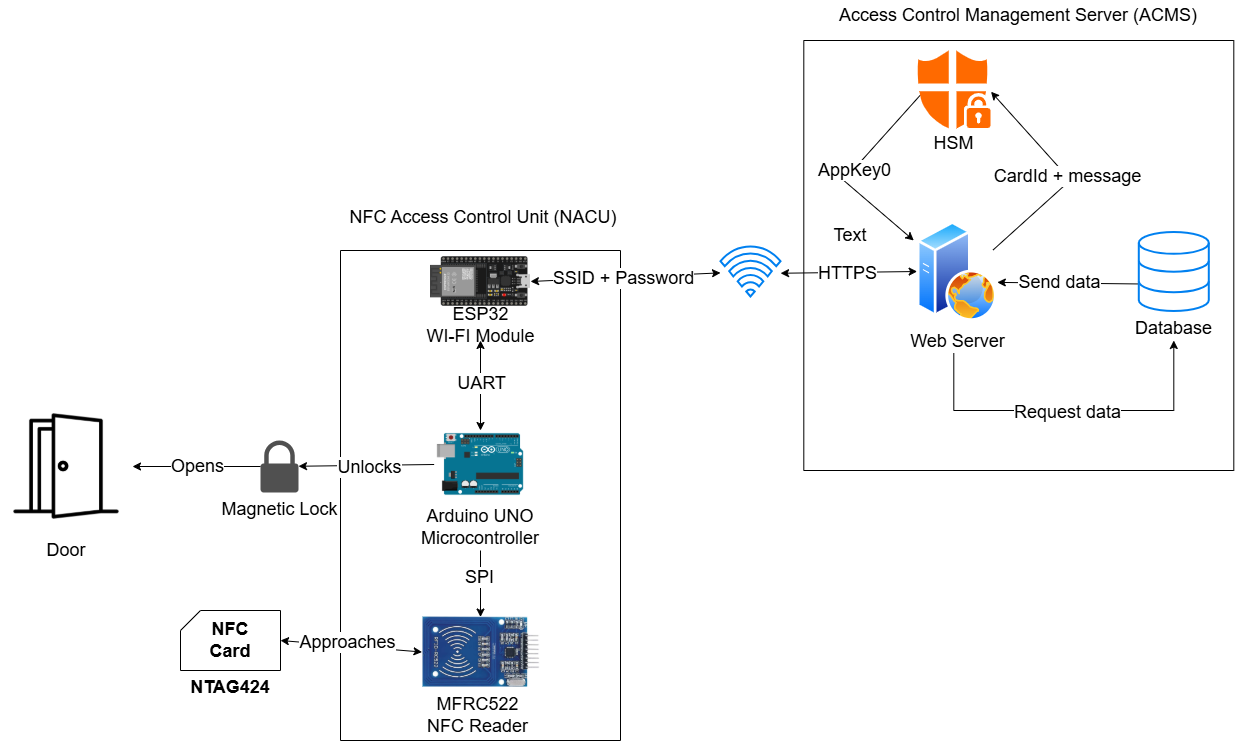
\includegraphics[width=\textwidth]{imaxes/Arqu.png}
	\caption{NFC Physical Access Control System Architecture. Left part of the figure represents the physical door with a
		magnetic lock, connected with the NACU module with an NFC Reader. The right part represents the ACMS server
		authentication module}
	\label{fig:arch}
\end{figure}

\subsection{Personal Authentication Data Flow}

When the users arrive at the physical facility and want to unlock the door to gain
access they tap their personal NFC card on the reader to identify themselves,
starting the personal authentication data flow. This Implementation employs the
ISO/IEC 14443‑4 EV2 mutual‑authentication protocol to verify the card’s authenticity
before proceeding with UID reading. 

Figure~\ref{fig:flow_auth}  describes the designed personal authentication protocol data flow, that summarizes the following operation:

\begin{enumerate}
	\item It starts as soon as the card approaches the NFC Access Control Unit
	(NACU).
	\item The reader, instead of first requesting an application key, reads directly the card identifier (CardId) stored in the NDEF file in Plain mode.
	\item The NACU sends to the Access Control Management Server (ACMS) a
	request including the CardId and a contextual message (“READUIDN”) that
	allows to differentiate the origin of the request.
	\item The server forwards this information to the HSM module, which computes an
	HMAC-SHA256 on the CardId and the message using the MasterKey and
	returns a 16 bytes AppKey0 to the ACMS, which forwards it to the NACU.
	\item With AppKey0 the protected reading procedure of the card UID is unlocked
	using the EV2 mutual authentication protocol, finally obtaining the UID.
	\item This UID is sent back to the ACMS, which compares it with its database of
	users and time slots to decide whether to authorize or deny access, returning
	the result to the NACU.
\end{enumerate}

\begin{figure}[H]
	\centering
	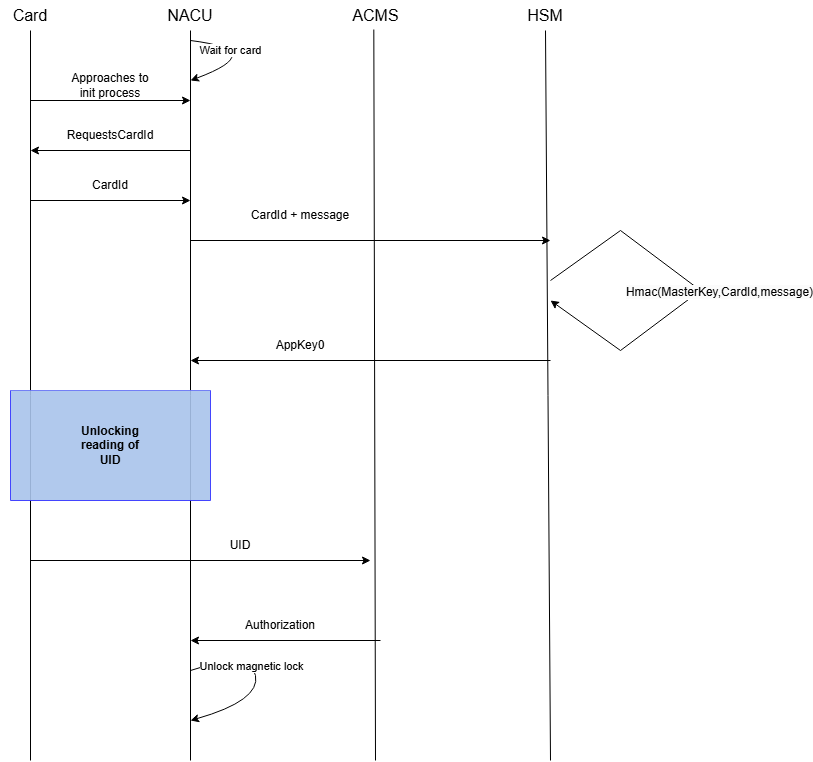
\includegraphics[width=\textwidth]{imaxes/DataFlow}
	\caption{General Personal Authentication Data Flow of the Final System, from the Approach of the card to the NACU, to the final Authorization}
	\label{fig:flow_auth}
\end{figure}

In Figure ~\ref{fig:nacu_states}  it is shown how each step of the data flow is managed as a different state as a loop in the microcontroller, so that the system proceeds in an orderly
fashion from card detection to final authorization, ensuring that each action is
executed only when appropriate within the defined flow. When a card is tapped, the
NACU sends its CardId to the ACMS and waits for the derived AppKey0. It then
receives AppKey0 and uses it to securely read the UID and send it to the ACMS.
Depending on the authorization ACMS response, the magnetic lock opens or
remains closed and the process ends. At each state in which a response from ACMS
is expected, a timeout ensures the reader resets and remains operational in case of
communication failure.

\begin{figure}[H]
	\centering
	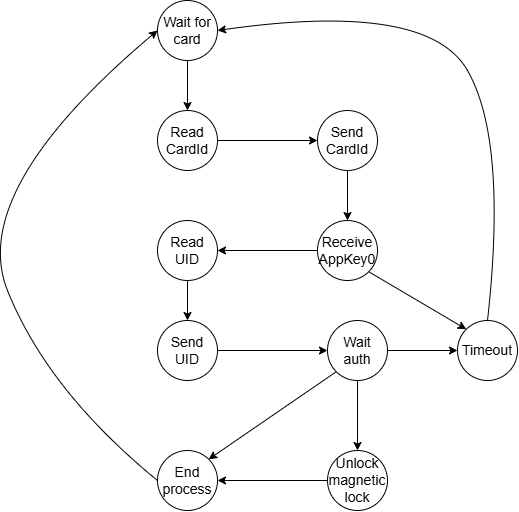
\includegraphics[width=\textwidth]{imaxes/stateD}
	\caption{ NACU state diagram for personal authentication using NFC cards}
	\label{fig:nacu_states}
\end{figure}

\subsection{Key Management System}

The system developed in this project employs a hierarchical and diversified key
management scheme (Figure~\ref{fig:key_management}), according to the strategy recommended by NXP
for the NTAG424 DNA \cite{ref42}. Each NTAG424 DNA card has a unique MasterKey,
which does not leave the trusted environment and is used only to derive four
application keys (AppKey0-AppKey3) that enable the different functionalities
available in FULL mode (\ref{subsec:keymanagement}).


The root of the hierarchy is the MasterKey, a 16-byte AES-128 value that resides
only within a Hardware Security Module (HSM). In a productive scenario, this HSM
would be a physical device that guarantees the inviolability of the key, but in this
academic prototype it is software simulated by a SoftHSM instance. The application
keys (AppKeys) are derived from the MasterKey using the HMAC-SHA256 function.
Also, each AppKey is assigned a “version number” (1 byte) that is incremented when
the key is updated, facilitating version identification and selective revocation. Thanks
to this hierarchical model, if an attacker managed to extract a specific AppKey from
the card, he would not be able to calculate the rest of the keys or the MasterKey, as
the derivation only works downstream.

AppKeyN is generated by applying a key derivation scheme based on
HMAC-SHA256 on the MasterKey and a specific context, and then truncating the
result to 128 bits. By truncating the HMAC we can obtain secure and distinct 128-bit
keys for each combination of context and card, ensuring that each AppKey is bound
to its intended use and is not reusable in other scenarios. However, for AppKey0, the
message used means to provide context using the format “READUIDN”, that
identifies to which reader or authentication station the request is addressed. This
variant allows the key to be associated with a specific reader, preventing AppKey0
from operating on unauthorized equipment.

Also, NTAG 424 DNA cards incorporate a protected hardware cryptographic storage
area (called “Key Store” or “Key Set”) \cite{ref29} in which AES keys are not directly
accessible by reading. These keys are located inside the chip's internal secure area
and can only be used through the encrypted EV2 authentication commands (e.g.
AuthenticateEV2First and AuthenticateEV2NonFirst), which implement a mutual
AES-128 challenge-response protocol.

At no step of the data reading or writing process does the key appear in the clear
over the RF channel: the values are encrypted before leaving the chip and are never
exposed externally. Therefore, even generic RF(radio frequency) devices such as a
Flipper Zero \cite{ref51} cannot extract or intercept them. Additionally, keys can have key
versions that invalidate any data obtained in previous attempts, forcing an attacker to
need knowledge of the current authentication key and correctly execute the EV2
protocol to modify or read protected files. In summary, the combination of secure
hardware storage, end-to-end encrypted communications and key version updates
makes it infeasible to steal or clone AppKeys or the MasterKey using commercial
NFC/RFID hacking equipment.
\begin{figure}[H]
	\centering
	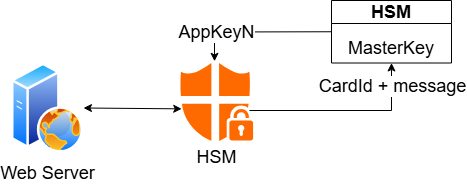
\includegraphics[width=\textwidth]{imaxes/KEY_MANA}
	\caption{Diagrama del sistema de gestión de claves. A la izquierda se representa la memoria de la tarjeta con NDEF y el conjunto protegido de claves, junto con la NACU y el ACMS.}
	\label{fig:key_management}
\end{figure}

\section{Initial prototyping and hardware assembly}
\label{sec:NACU1}

In the initial prototyping phase, the primary objective is to assemble, configure and rigorously validate the hardware components that constitute the access control system using an iterative approach. An Arduino Uno was selected as the main microcontroller to orchestrate sensor and actuator operations, while an ESP32 module provides IEEE 802.11 Wi-Fi and Bluetooth connectivity for bidirectional data exchange with the ACMS \cite{ref45}. NFC functionality is handled by the MFRC522 module, which supports both reading and writing functionalities with NTAG cards.

Seamless interoperability among these devices is essential for establishing a robust, low-latency communication backbone. Accordingly, each component is mounted on a solderless breadboard and interconnected in accordance with the best wiring practices. Comprehensive configuration and functional testing at this stage lay the groundwork for subsequent software integration and the enforcement of cryptographic security protocols.

\subsection{NFC Reader Integration with the Microcontroller}

The MFRC522 module provides two communication interfaces with the Arduino UNO: Serial Peripheral Interface (SPI) and Inter-Integrated Circuit (I2C), operating solely at 3.3 V to guarantee electrical compatibility with the microcontroller. The SPI interface was chosen for this project due to its higher transfer speeds and ease of implementation in prototyping environments.

The physical interconnection was created by soldering the wires according to the following pin diagram (Figure \ref{fig:MFRC-ArduinoUno}):

\begin{table}[H]
	\centering
	\begin{tabular}{|c|c|}
		\hline
		\textbf{MFRC522 PINS} & \textbf{Arduino Uno PINS} \\
		\hline
		3.3V & 3.3V \\
		GND & GND \\
		RST & 9 \\
		SDA & 10 \\
		MOSI & 11 \\
		MISO & 12 \\
		SCK & 13 \\
		\hline
	\end{tabular}
	\caption{MFRC522-Arduino UNO Wiring Following the SPI standard}
	\label{tab:mfrc522_arduino}
\end{table}

\begin{figure}[H]
	\centering
	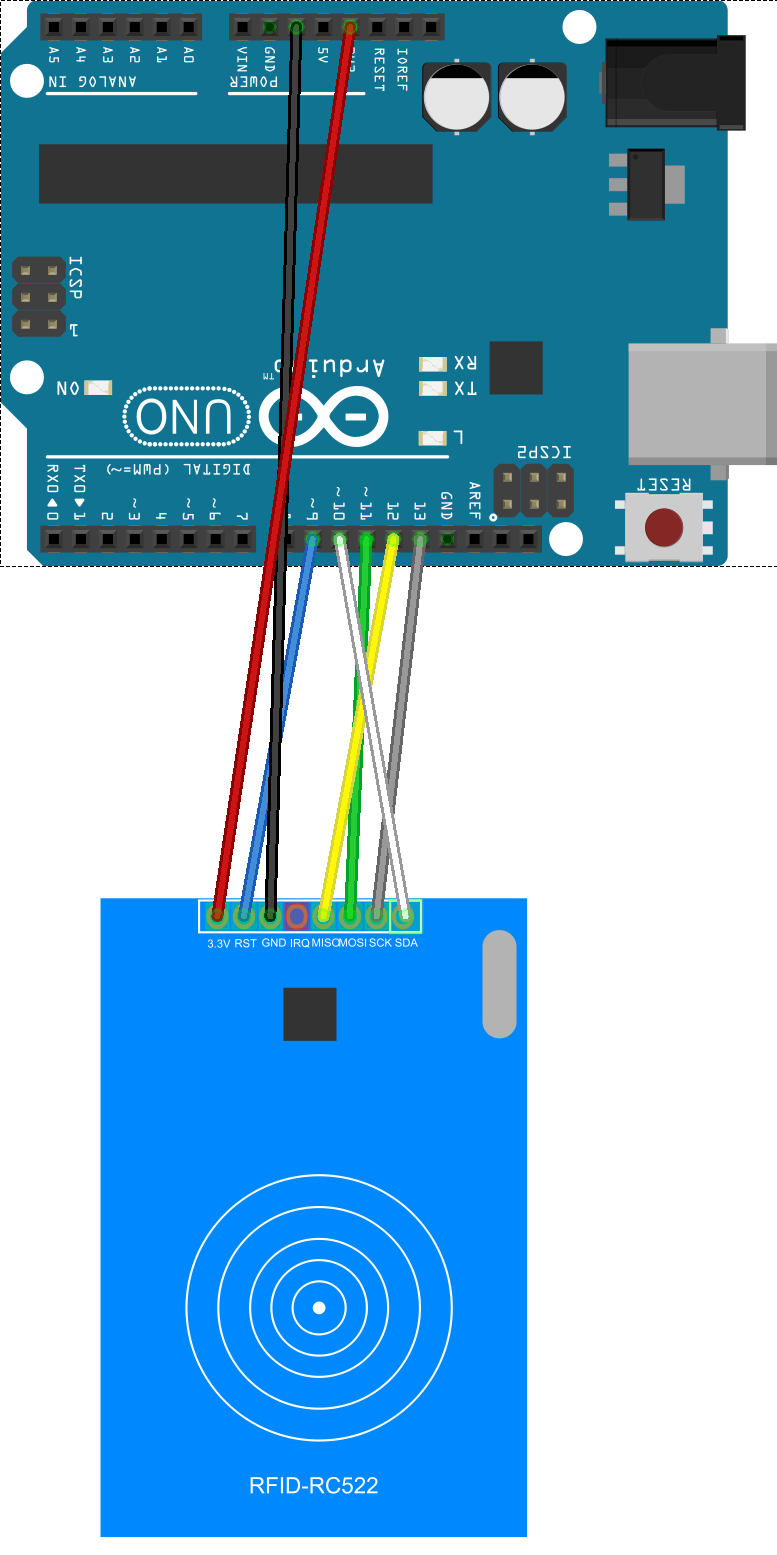
\includegraphics[width=0.5\textwidth]{imaxes/UNOMFRC}
	\caption{MFRC522-ArduinoUNO Wiring Following the SPI standart}
	\label{fig:MFRC-ArduinoUno}
\end{figure}

To validate all cryptographic functionalities of the NTAG424 DNA, the MFRC522\_NTAG424DNA library itself provides a series of test sketches. For each functionality there are three levels of security:

\begin{itemize}
	\item \textbf{PLAIN}: clear text communication.
	\item \textbf{MAC}: adds a message authentication code (MAC) calculated with AES-128, guaranteeing the integrity and authenticity of the commands, but without encrypting the content.
	\item \textbf{FULL}: establishes an end-to-end encrypted channel following an EV2 mutual authentication protocol with AES-128, protecting the confidentiality of all data exchanged \cite{ref42}.
\end{itemize}

\subsection{Wi-Fi module integration}

The ESP32 module provides Wi-Fi and Bluetooth connectivity, forming the bridge between the NFC Access Control Unit (NACU) and the Access Control Management Server (ACMS). To ensure the reliability of the data flow from the Arduino UNO to the ESP32, the serial interconnection is verified before integrating any network logic. The interface chosen is UART (Universal Asynchronous Receiver-Transmitter), due to its wide compatibility, low resource consumption and the need for only two data signals.

It is important to note that the default UART port of the Arduino UNO (pins 0 and 1) is reserved for communication with the computer during sketch loading. Therefore, two additional digital pins and the \texttt{SoftwareSerial} object are used to avoid interference with the USB programmer. Also, the same issue is encountered when configuring this protocol in ESP32, the UART0 (GPIO 1: TX0, GPIO 3: RX0) is reserved for connection to the computer, both for firmware upload and serial monitor, so it should not be used for communication with the Arduino UNO.

Therefore, pin connections are established as follows (Figure \ref{fig:ESP32-ArduinoUno}):

\begin{table}[H]
	\centering
	\begin{tabular}{|c|c|}
		\hline
		\textbf{Arduino UNO pins} & \textbf{ESP32 pins} \\
		\hline
		2 (TX) & 27 (RX) \\
		3 (RX) & 26 (TX) \\
		\hline
	\end{tabular}
	\caption{ESP32-Arduino UNO Wiring Following the UART standard}
	\label{tab:esp32_arduino_uart}
\end{table}

\begin{figure}[H]
	\centering
	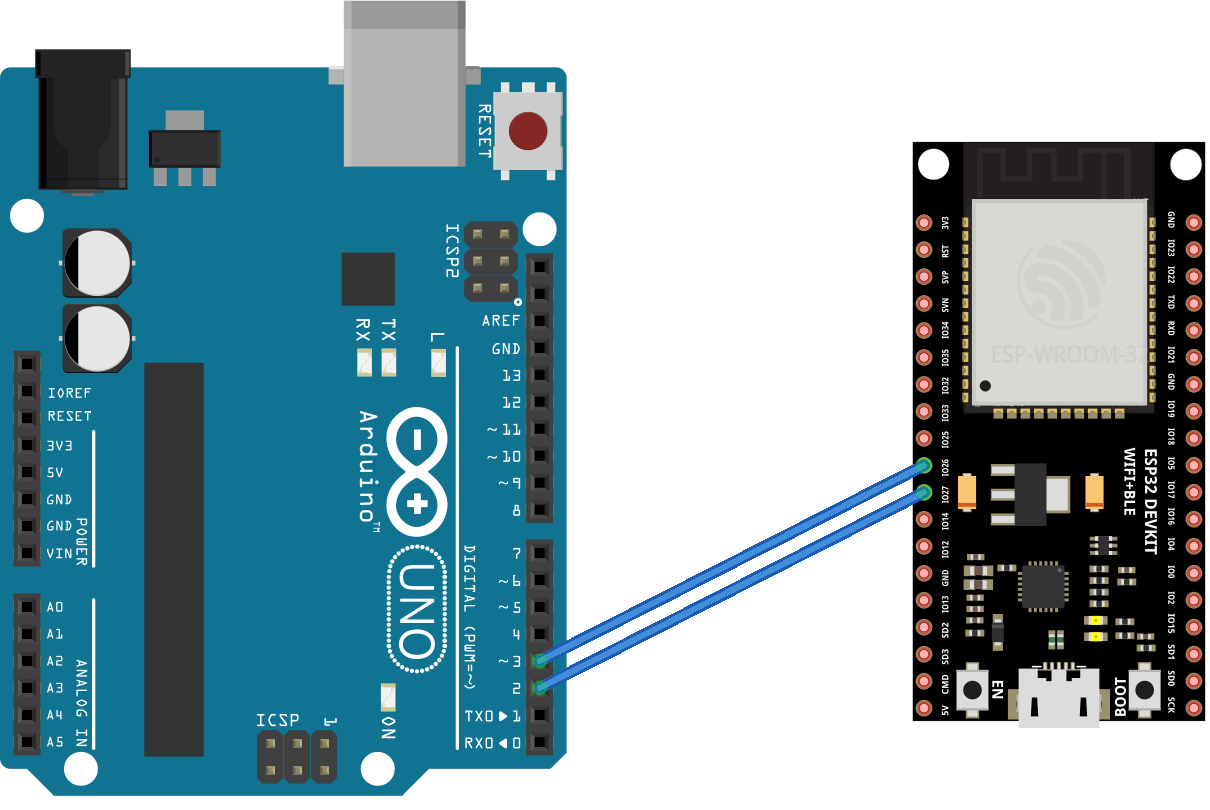
\includegraphics[width=\textwidth]{imaxes/esp32UNO}
	\caption{ESP32-ArduinoUNO Wiring Following the UART standard}
	\label{fig:ESP32-ArduinoUno}
\end{figure}


Each module receives independent power through its connectors, ensuring stability and electrical isolation. Once this UART transport layer is established, access control protocols and HSM commands can be implemented on it without risk of data loss or overlapping.

\subsection{Physical lock integration}


To incorporate the LIBO 12 V/180 kg magnetic lock into the access control prototype, a Dollatek DC 0-5 V relay module is used to interface between the Arduino Uno and the 12 V power supply of the lock (Figure: \ref{fig:maglock_arduino}).

For supplying the relay, 5 V and GND connections from the Arduino Uno are connected to the V\textsubscript{CC} and GND pins of the relay module, respectively. Digital pin DN (configurable in the sketch) goes to the IN pin of the relay.

Also, for powering the lock, the 12 V 1.5 A adapter provides power to the magnetic coil. Its +12 V pole connects to the COM terminal of the relay; the GND of the adapter connects to the return power terminal of the lock.

The NO (Normally Open) terminal of the relay goes to the positive power terminal of the lock. When the relay is activated, it closes the circuit between COM and NO and energizes the coil.

\begin{figure}[H]
	\centering
	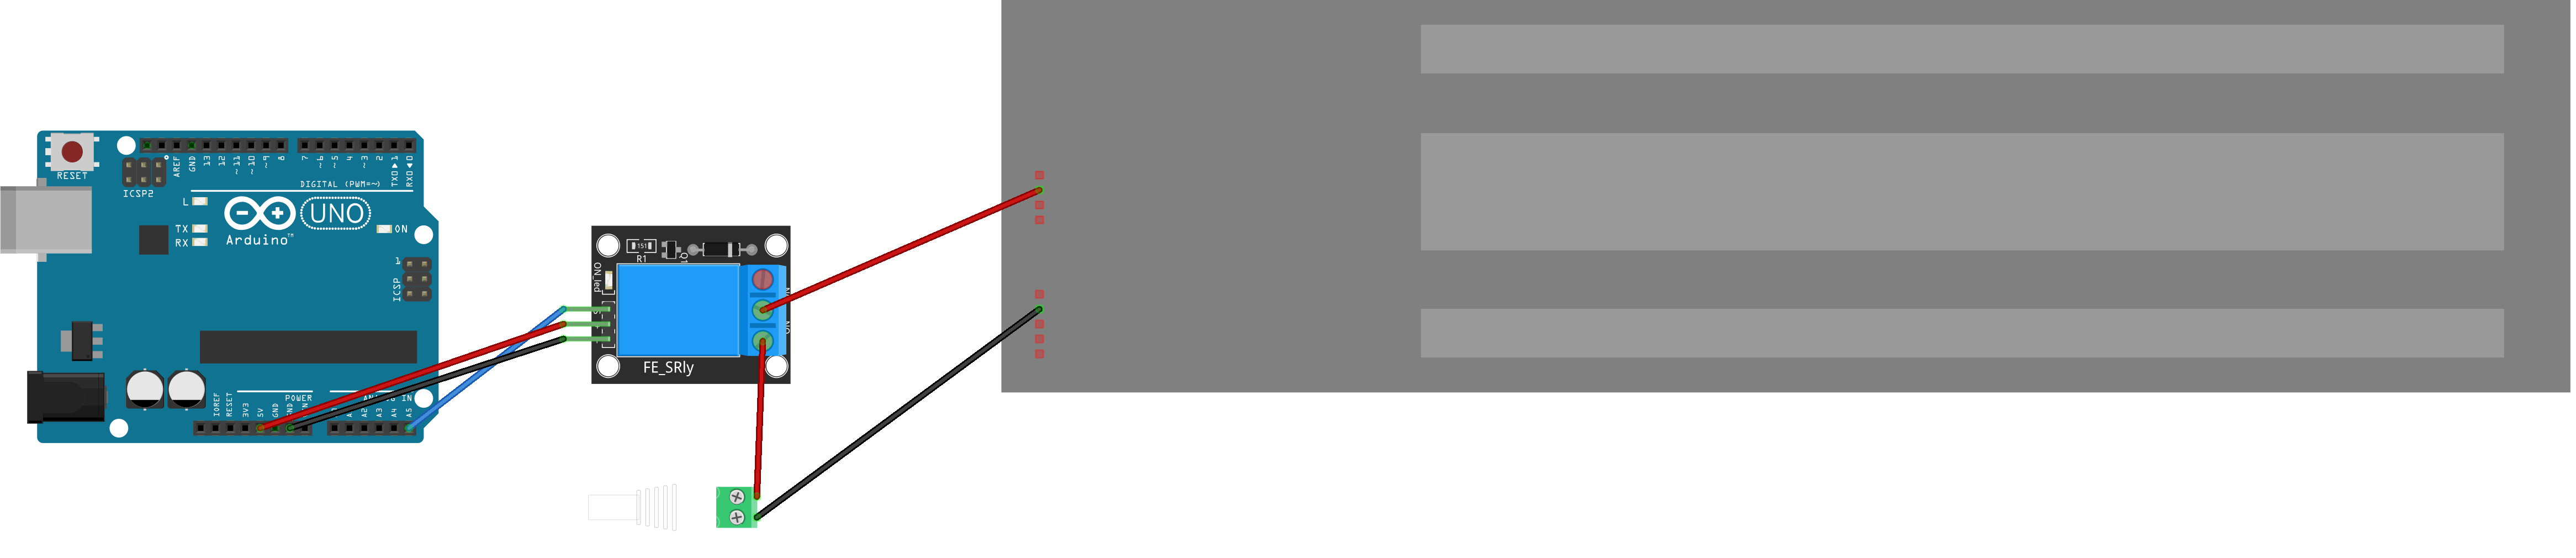
\includegraphics[width=0.7\textwidth]{imaxes/maglock.png}
	\caption{Maglock-Arduino UNO Wiring, with the Arduino connected via 5 V and GND pins for power management to a relay, which obtains power from the voltage adapter to redirect it to the magnetic lock (shown on the right).}
	\label{fig:maglock_arduino}
\end{figure}

\section{NFC Access Control Unit (NACU)}
\label{sec:NACU2}

The objective of this section is to describe how the modular hardware part of the system is created using an iterative scope. In each step, a new module is added and its ability to communicate with the already‑tested modules is verified using the relevant protocol so that by the end of the cycle every hardware element has been proven capable of interoperating reliably under the conditions it will face in the completed system.

\subsection{Iteration 1: Basic NFC communication}

The objective of this iteration is to establish reliable communication between the NFC reader (MFRC522) and the NTAG 424 DNA card, enabling secure extraction of its unique identifier (UID) in “Full” mode (ISO 14443-4) \cite{Ref65}. This iteration lays the foundation for subsequent authentication and key management phases.

Before running any test, the firmware must perform two generic tasks:
\begin{itemize}
	\item The SPI interface is initialized to communicate the microcontroller (Arduino Uno) with the MFRC522 module and the reader performs a software reset.
	\item Each loop verifies that the reader detects a valid card (“OK” status) before proceeding to the next step, thus ensuring that all subsequent operations are performed only when the hardware is ready and the card responds correctly.
\end{itemize}


During this iteration, the wires had to be welded in for the NFC communication to be constant.

\subsubsection{Secure NFC card UID Reading}

In the verification of the NTAG424 DNA UID‐reading functionality, the example sketch \texttt{Full\_GetCardUID} provided by the MFRC522\_NTAG424DNA library is employed as a reference implementation. 

Before each critical operation, the system checks a status code to ensure that the previous step has been completed successfully (“DNA\_STATUS\_OK”). If there is a failure, it returns to the start of the cycle and waits for a card again.

The flow needed to securely read the UID using the library standard is represented in Figure \ref{fig:5.8}:
\begin{enumerate}
	\item The NFC reader identifies that a new card has entered its field and resolves possible collisions to always work with a single tag.
	\item The correct memory area inside the NTAG424 card is accessed for protected operations.
	\item A secure channel via EV2 (Enhanced Version 2) mutual authentication is established using AppKey0.
	\item The 7-byte unique identifier of the card is retrieved under the secure channel, ensuring its confidentiality and integrity.
	\item Finally, the decrypted UID is sent to the serial monitor.
\end{enumerate}

\begin{figure}[htbp]
	\centering
	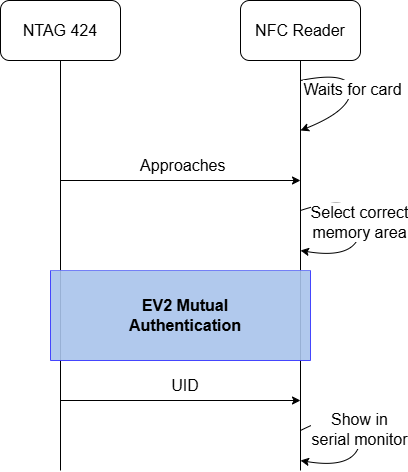
\includegraphics[width=0.6\textwidth]{imaxes/UID_READ} % Añade aquí la ruta de la figura
	\caption{NTAG424 card UID Read after performing mutual authentication with NFC Reader}
	\label{fig:5.8}
\end{figure}

\subsection{Iteration 2: Providing basic Wi-Fi connectivity}

The objective of this iteration is to create a bi-directional, stand-alone communication channel between the Arduino Uno (which manages the NFC reader) and the ESP32 (which connects to the server), without occupying or interfering with the ESP32's USB programming port. This keeps the USB port free for firmware uploads and debugging, while ensuring reliable data exchange between the two microcontrollers.

To ensure proper communication between the computer and the ESP32 module through the Arduino IDE development environment, it is necessary to first proceed with the installation of the corresponding USB-UART driver. In this case, the Silicon Labs CP210x chip is the serial bridge used by most ESP32-based boards, so the “CP210x VCP Drivers” \cite{ref46} driver package must be installed in the operating system. These drivers allow the system to recognize the USB device as a virtual serial port (VCP), enabling program loading and serial monitoring.

Once the driver is installed, the ESP32 is configured within the Arduino IDE. To do it, the official “esp32” plug-in is added in the Board Manager via the URL provided by Espressif Systems. This package includes both the cross-compilation drivers (toolchains) and the libraries necessary for the IDE to detect and program the ESP32 board. After completing this step, any test sketch can be loaded into the module.

In order to test the serial communication between the microcontroller and the WI-FI module, a sketch is uploaded, with the purpose of sending a simple message and displaying it in the serial monitor. In order to perform this task, UART protocol is used via pins RX and TX 2 and 3 in the microcontroller and GPIO 27 and 26 respectively in the WI-FI module. The microcontroller uses the serial bus communication for sending a test message, while the WI-FI module checks whether the channel is free, and then proceeds to listen to it until a space (“\textbackslash n”) is found (Figure \ref{fig:5.9}).

\begin{figure}[htbp]
	\centering
	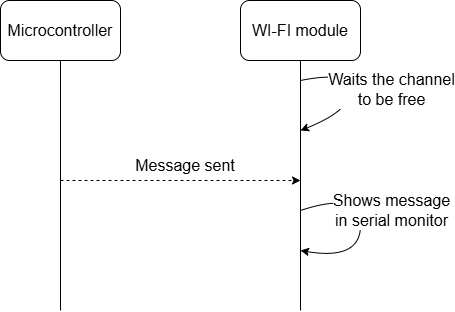
\includegraphics[width=0.6\textwidth]{imaxes/MICROCONTROLLERESP32} % Añade aquí la ruta de la figura
	\caption{ESP32 WI-Fi module Shows UART Message via Serial Monitor}
	\label{fig:5.9}
\end{figure}

\subsection{Iteration 3: Mutual authentication and configuring NFC card identifiers}

The objective of this iteration is to implement EV2 (Enhanced Version 2), which procedure is explained in Section \ref{subsec:EV2}, Full authentication and plain NDEF writing on NTAG424. During this phase, several NTAG424 features are tested, like status error handling, AES-128 handshake, retries on “deselectAndWakeupA” and random challenges generation optimization. Also, writing arbitrary data to the NDEF file raised awareness on the correct setting of offsets and maximum block length for this process to work. In addition, memory cleanup to avoid leaks and buffer management was implemented.

\subsubsection{EV2 Mutual Authentication with AppKey}

The EV2 protocol  in the NACU sketch it is implemented the following way:

\begin{enumerate}
	\item The reader creates a 16‑byte random challenge, RndA, by sampling an entropy source (e.g. \texttt{randomSeed(analogRead(0))} on Arduino) inside the \texttt{generateRndA} function.
	\item It then encrypts RndA with AppKey0 and sends it to the tag to start the EV2 handshake.
	\item The underlying library takes over from there: it receives the tag’s encrypted response, checks that RndA matches the decrypted value (\ref{fig:3.2}), and completes the mutual‑authentication sequence.
\end{enumerate}

\subsubsection{Configuring NFC card identifiers}
\label{subsubsection:cardidload}
To enable uploading card identifiers (CardId) to the NDEF region of the unencrypted NTAG424 DNA card (Plain Mode), the following flow is implemented, inspired by the \texttt{Plain\_WriteData} example in the MFRC522\_NTAG424DNA library, as shown in Figure \ref{fig:5.10}:

\begin{enumerate}
	\item The NFC reader identifies that a new card has entered its field and resolves possible collisions to always work with a single tag.
	\item Then, parameters such as the target file, the position where the data will be written, and the content to be stored are defined.
	\item The serial console printout confirms success or reports the error code (st) in case of failure, allowing to immediately validate if the card stores the NDEF section correctly.
\end{enumerate}

\begin{figure}[htbp]
	\centering
	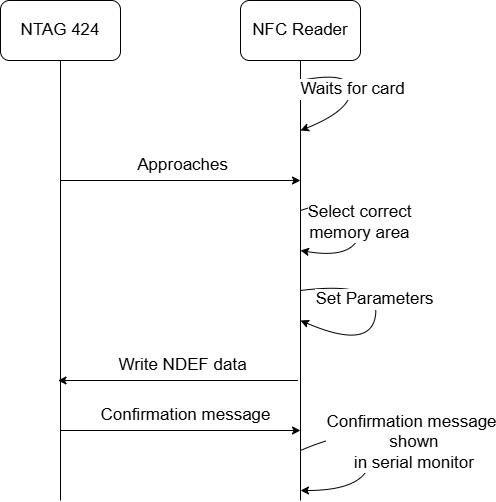
\includegraphics[width=0.6\textwidth]{imaxes/NDEFWIRTE} % Añade aquí la ruta de la figura
	\caption{NTAG 424 NDEF memory file Writing in Plain Mode}
	\label{fig:5.10}
\end{figure}

\subsection{Iteration 4: Reading NFC Card memory and Loading Cryptographic Keys}

The objective of this iteration is to read arbitrary data from the NDEF file and test the key change feature from NTAG424, which is protected by EV2 mutual authentication with the MasterKey.

\subsubsection{Obtaining NFC card identifiers}

One of the fundamental steps to validate system operation is to test the NACU's ability to retrieve data stored on an NTAG424 DNA card. This card has multiple internal files, among which the NDEF (NFC Data Exchange Format) file is commonly used to store structured information readable by NFC compatible devices. In this system, a card identifier is stored in it, and must be retrieved during the personal identification process.

In order to perform basic reading without applying advanced cryptographic authentication, we have chosen to operate in Plain communication mode. This mode allows reading operations to be performed without the need for a prior mutual authentication procedure or channel encryption.

To enable reading data from the NDEF memory region of the NTAG424 DNA on Plain Mode, the following procedure is followed based on the \texttt{Plain\_ReadData} sample sketch from the MFRC522\_NTAG424DNA library, in which after a card is selected and detected(FIgure \ref{fig:5.11}):
\begin{enumerate}
	\item The application designates the NDEF memory area on the card and specifies how many bytes to read.
	\item The NDEF file’s contents are retrieved in clear text and stored in a temporary buffer.
	\item The serial monitor confirms whether the information stored in the buffer is correct.
\end{enumerate}

\begin{figure}[htbp]
	\centering
	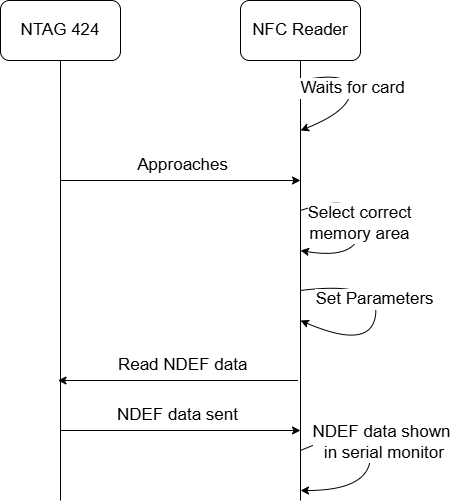
\includegraphics[width=0.6\textwidth]{imaxes/NDEF_READ} % Añade aquí la ruta de la figura
	\caption{NTAG 424 NDEF memory file reading in Plain Mode}
	\label{fig:5.11}
\end{figure}

\subsubsection{Key loading into the NFC card}
\label{subsubsection:keyload}
To securely update any of the keys stored in an NTAG424 DNA it is necessary to use the EV2 protocol (AES-128 mutual authentication) and the \texttt{DNA\_Full\_ChangeKey} function of the MFRC522\_NTAG424DNA library as shown in Figure \ref{fig:5.12}:
\begin{enumerate}
	\item The MasterKey is used in the EV2 mutual authentication.
	\item Then, a new key is defined using:
	\begin{enumerate}
		\item \texttt{keyNumberToChange} selects the AppKey to be used as the target of the update.
		\item \texttt{newKey} as the 16-byte array with the desired new value.
		\item \texttt{newKeyVersion}, a byte that increments the internal version, allowing to manage key versions.
	\end{enumerate}
	\item Finally, the key is changed using the \texttt{DNA\_Full\_ChangeKey} function and validated through the serial monitor.
\end{enumerate}

\begin{figure}[H]
	\centering
	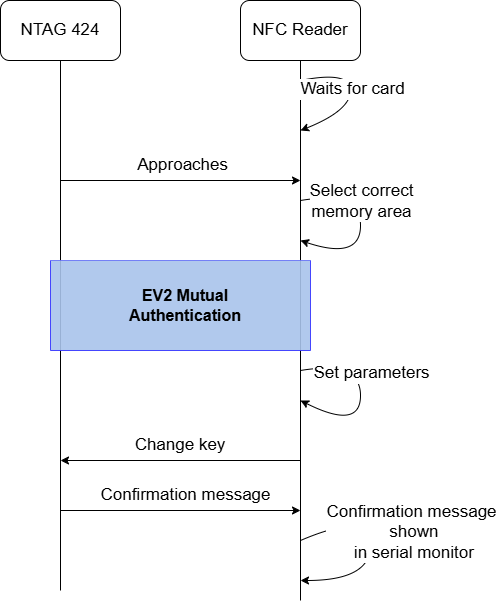
\includegraphics[width=0.6\textwidth]{imaxes/KEYCANGE} % Añade aquí la ruta de la figura
	\caption{Change of NFC NTAG424 card AppKey1, which needs EV2 mutual authentication}
	\label{fig:5.12}
\end{figure}

\subsection{Iteration 5: NACU Subsystem Full Integration}

The objective of this iteration is to connect UID reading with ESP32, for later sending the UID to the ACMS. In order to achieve it, sketches must be consolidated, elaboration of single flow with test scripts of Wi-Fi module and microcontroller. To validate the end-to-end flow, NFC reader obtains the UID of a NTAG424 card, microcontroller sends it over UART and WI-FI module checks its arrival via serial monitor.

\subsubsection{Card UID and AES Key Transfer between NACU modules}

To verify the UART data flow that is used in the final product, the UID of an NTAG424 DNA card is read in “plain” (unencrypted) mode and forwarded by the microcontroller by the UART port to the WI-FI module, which receives it and displays it on the screen as in the previous test. In this way, we verify that the board identifier is reliably transmitted along the system (Figure \ref{fig:5.13}).

\begin{figure}[htbp]
	\centering
	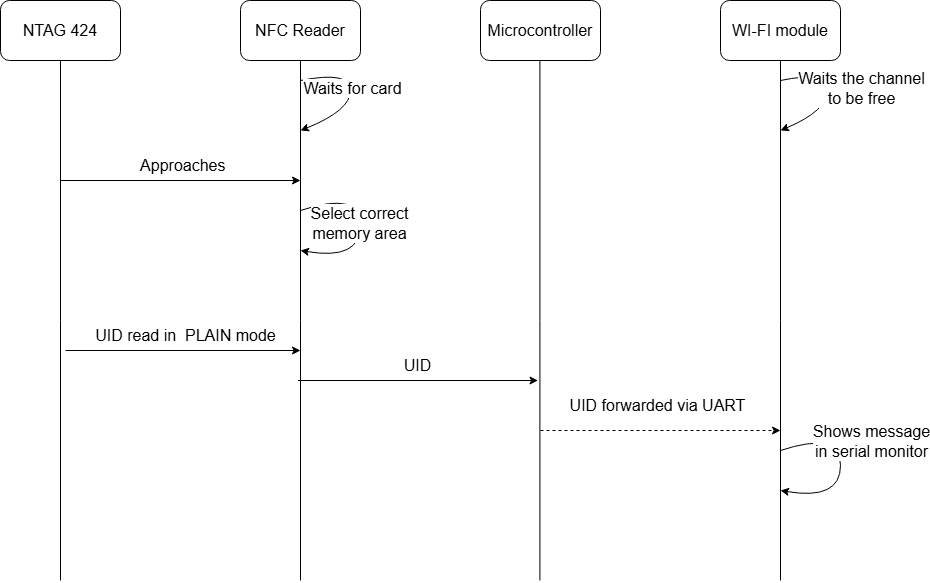
\includegraphics[width=\textwidth]{imaxes/FINALFLOW} % Añade aquí la ruta de la figura
	\caption{ESP32 Wi-FI module receiving via UART NTAG 424 UID after plain read performed by the NFC Reader}
	\label{fig:5.13}
\end{figure}

Also, in order to validate the transmission of fixed-length binary data backwards, the Wi-FI module sends via UART an AES-128 key (AppKey) as a 16-byte array. On the microcontroller, a sketch similar to the one for receiving the UID is executed: it reads exactly 16 bytes from the serial port, displays them on the monitor and uses this key to perform mutual authentication in a compatible card using the NFC reader. 


\subsection{Iteration 6: Magnetic lock Management for Physical Access Control}

The objective of this iteration is to implement the logic to integrate the Maglock in the system. This component only needs to communicate with the Arduino Uno, which must control the voltage in order to manage the unlocking of the Maglock when needed.

For performing this action, one analog pin from the Arduino Uno must be connected to the relay, and in the \texttt{setup()} part of the code its voltage must be set to HIGH in order to lock it. Then, when the situation is needed, the voltage of this pin must be set to LOW in order to unlock it.


\section{Access Control Management Server (ACMS)}
\label{sec:ACMS}

The objective of this section is to create a backend administration server using an incremental approach. The Django~\cite{Ref20} framework was chosen for this task because the Model‑View‑Controller~\cite{Ref61} architecture, combined with a built-in admin and login interface provides the scalability, security, and rapid‑development capabilities best suited to the project needs.

\subsection{Iteration 1: Basic Structure and Authentication}

The objective of this iteration is to provide the ACMS with a strong basis by implementing a RESTful API and a robust authentication system. These foundations will allow, in successive iterations, to incrementally incorporate the specific functionalities needed to complete the entire access control flow.

\subsubsection{Time Window Based Access Control and Auditory}

First, an internal application called \texttt{core} was created to encapsulate all the specific logic for access control and communication with the NFC Access Control Unit (NACU). Django follows the Model-View-Template (MVT) pattern, so the first step was to define the models that would represent the domain entities in the data layer. All of them were declared in \texttt{core/models.py} and registered in the administration panel through \texttt{core/admin.py}, which facilitates the management of users, schedules and keys directly from the Django Admin interface. The most relevant model classes were:

\begin{itemize}
	\item \textbf{HSMData}: Stores personal data associated with the user and the card UID linked to him.
	\item \textbf{AccessLog}: Logs each access attempt, storing the UID sent, the user's name (related to the corresponding entry in HSMData) and the timestamp of the event. In addition, an \texttt{authorized} boolean field was included indicating whether access was granted according to the configured schedule.
	\item \textbf{EntrySchedule}: Allows defining the valid access time slots for each user, linked to the HSMData entity.
\end{itemize}

Once these models were defined, the framework's own migrations were executed with the \texttt{makemigrations} and \texttt{migrate} commands, synchronizing the definition of the tables in the database.

To provide visual consistency and facilitate the reuse of components in template-based views, a global template folder was set up in \texttt{settings.py} using the line \texttt{'DIRS': [BASE\_DIR / 'templates']}. From here, a base file (\texttt{base.html}) was implemented to serve as a common template for all views, and specific templates \texttt{login.html} and \texttt{log\_list.html} were generated to extend \texttt{base.html} to cover the different functionalities of the system. As for the views and routes layer, the fundamental REST endpoints were defined in \texttt{core/views.py} (Figure~\ref{fig:mvc-schema}).

\begin{figure}[H]
	\centering
	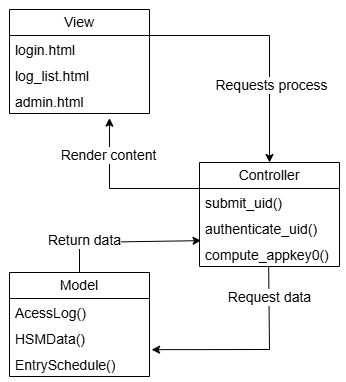
\includegraphics[width=0.75\textwidth]{imaxes/MVC.png}
	\caption{MVC Schema Representing the Views, that are managed by the Controller, that extracts data from the Model}
	\label{fig:mvc-schema}
\end{figure}

\subsubsection{Access Control Endpoints for Administration and NACU Communication}

In this section the three HTTP endpoints that form the core API between the NFC access control units (NACU) and the Access Control Management Server (ACMS) are defined. Together they handle every card‐based access attempt, recording each try, validating against registered UIDs and time schedules, and automating alerts, while also providing an interface for administrators.

\begin{itemize}
	\item \textbf{/submit\_uid/ (POST/GET)}
	\begin{itemize}
		\item Receives the NFC card UID.
		\item Immediately saves an attempt record.
		\item Checks if the UID exists and, if it does, validates if it is within its authorized schedule.
		\item Updates the log with the result and, if not allowed, triggers a mail alert.
	\end{itemize}
	
	\item \textbf{/authenticate\_uid/ (GET)}
	\begin{itemize}
		\item Verifies the existence and schedule of the UID.
		\item Logs the result.
		\item Redirects to view where all access logs are displayed.
	\end{itemize}
	
	\item \textbf{/log\_list/ (GET)}
	\begin{itemize}
		\item Retrieves all logs.
		\item Renders the view for administrators to review.
	\end{itemize}
\end{itemize}

\subsection{Iteration 2: Key Derivation System}

In this second iteration, the objective is to deploy and configure a Hardware Security Module (HSM) in software, and to create in the ACMS an endpoint that, from a \texttt{CardId} and a \texttt{message}, generates the \texttt{AppKey0} key using HMAC-SHA256.

\subsubsection{Hardware Security Module Implementation}

In the system, the Master Key plays a key role in terms of security. It is not only used to load the AppKeys on each card, but also to derive all subsequent keys. Its compromise compromises the confidentiality of the entire infrastructure. For this reason, the Master Key must be given a higher level of protection than any other cryptographic credential.

For development and test environments, SoftHSM is used, a software-based HSM implementation that complies with the PKCS\#11~\cite{Ref76} specification. A slot in PKCS\#11 is a logical container that can hold a token. Before we can store keys, we must create and initialize that token on disk and assign it an administrator PIN (SO-PIN) and a user PIN. After uploading two different keys into the slot, the result is shown in Figure~\ref{fig:hsm-slots}.

\begin{figure}[H]
	\centering
	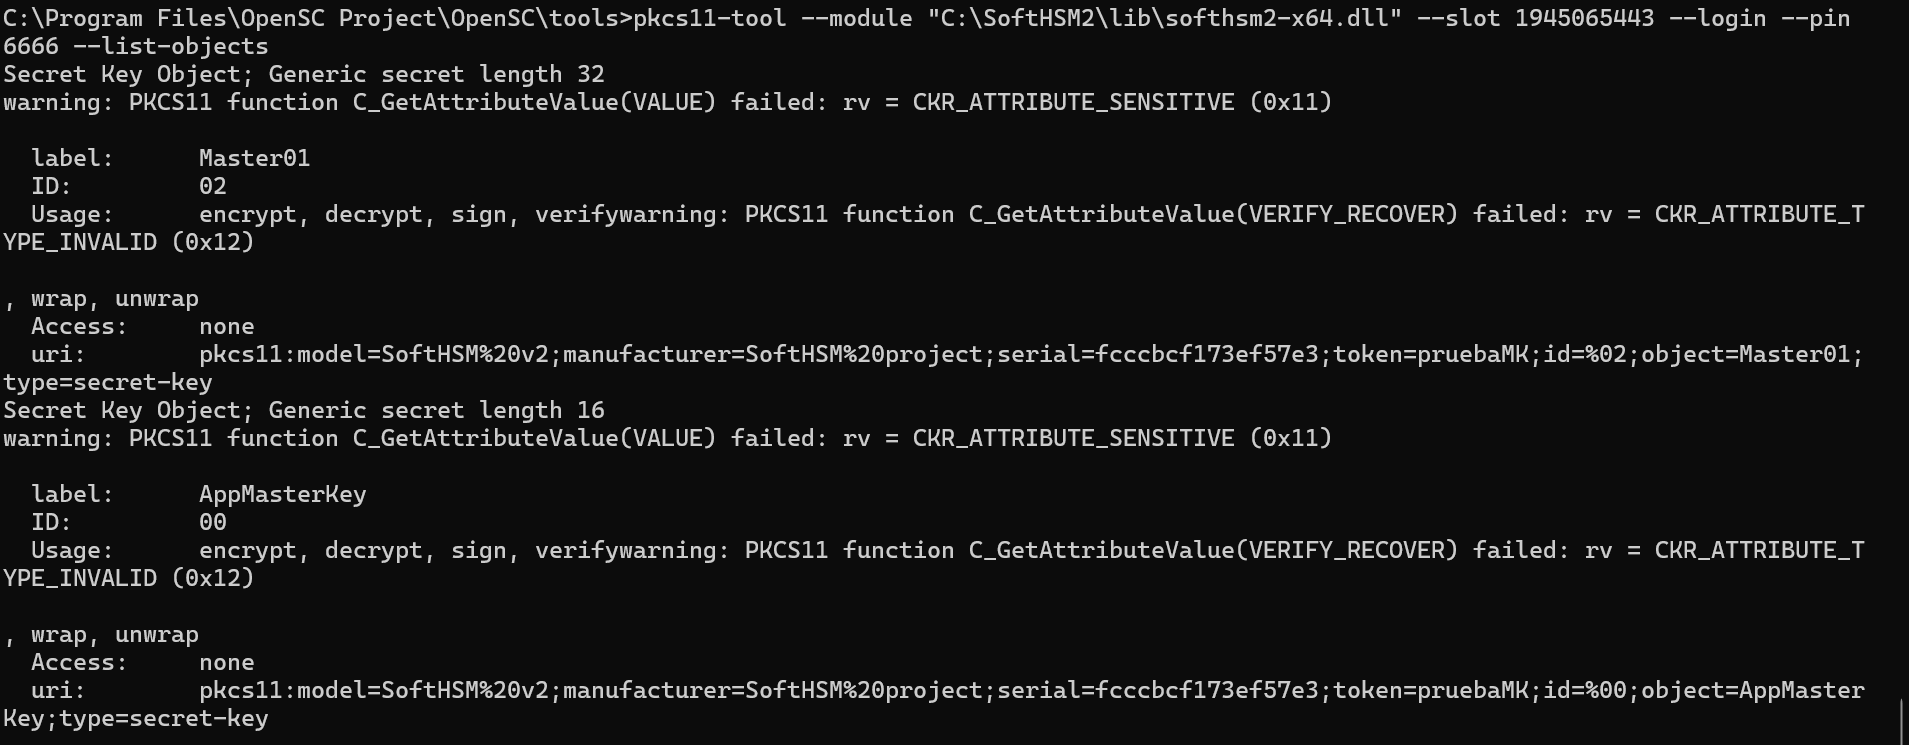
\includegraphics[width=\textwidth]{imaxes/hsm.png}
	\caption{Slots of HSM. Master01 and AppMasterKey are stored and labeled, with no access allowed and the type of object is secret-key}
	\label{fig:hsm-slots}
\end{figure}

\subsubsection{Key Derivation System Integration in ACMS}

To invoke the virtual HSM from Django, the \texttt{/compute\_appkey0/} endpoint dumps the concatenation \texttt{cardid\_bytes + msg} to disk and, via a subprocess invoking the same command used in CMD, requests the SoftHSM2 token to execute an HMAC-SHA256 with the Master Key. The PKCS\#11 module signs the input file and deposits the result in \texttt{OUTPUT\_PATH}. Django then opens this file, extracts the first 16 bytes of the HMAC and returns them as a hexadecimal string.

\subsubsection{Key Derivation Endpoint}

The purpose of the endpoint \texttt{/compute\_appkey0/} (GET) is to derive a 128-bit key (AppKey0) using HMAC-SHA256 on the \texttt{CardId} and a contextual message.

\textbf{Parameters:}
\begin{itemize}
	\item \texttt{CardId}: card identifier in hexadecimal (32 hex digits).
	\item \texttt{msg}: additional text string to be concatenated to the identifier.
\end{itemize}

\textbf{Main flow:}
\begin{enumerate}
	\item Validates presence of \texttt{CardId} and \texttt{msg}, returns 400 if missing.
	\item Converts \texttt{CardId} to bytes, returns 400 if format invalid.
	\item Concatenates bytes and writes to input file.
	\item Invokes \texttt{pkcs11-tool.exe} externally. Raises 500 on failure.
	\item Reads HMAC result and checks length.
	\item Extracts first 16 bytes and returns them as uppercase hex string.
\end{enumerate}


The endpoint uses \texttt{@csrf\_exempt} so NACU can call it directly. Any error returns HTTP 500 for immediate reader-side detection.


\subsection{Iteration 3: Transport encryption (HTTPS/TLS)}
\label{subsec:https}

The objective of this iteration is to increase the security of the ACMS for it to scale from HTTP, which is the default from Django, to HTTPS/TLS.

\subsubsection{ACMS Communication Encryption}

In order to guarantee the confidentiality and integrity of communications between the NACU and the Django server during the development phases, the server was scaled from HTTP to HTTPS using locally trusted self-signed certificates.

Django's \texttt{runserver} default command only exposes HTTP (no encryption). \texttt{Django-sslserver} \cite{Ref47} is a development extension that enables a temporary HTTPS server, suitable for local environments. Its use in production environments is not recommended, but it is ideal for end-to-end TLS verification in development.

\texttt{Mkcert} \cite{Ref48} is the command-line utility chosen to generate "locally trusted" X.509 certificates. It installs a private Certificate Authority (CA) in the operating system's certificate store, allowing you to quickly create valid TLS certificates for local IP addresses or domains without browser security warnings.

Also, in order to establish TLS/SSL connections from the NACU, Arduino IDE provides the \texttt{WiFiClientSecure} \cite{Ref49} library. It supports the encryption and negotiation process of the TLS protocol and can accept self-signed certificates if configured with \texttt{setInsecure()}. In addition, the \texttt{HTTPClient} \cite{Ref50} library is provided to facilitate making HTTP(S) requests over a \texttt{WiFiClient} or \texttt{WiFiClientSecure}.

\textbf{General flow:}
\begin{enumerate}
	\item Installation of the local CA. With Mkcert a Certificate Authority is created and imported into the system's certificate store. From then on, any certificate issued by that CA will be recognized as valid by the OS and local browsers.
	\item X.509 TLS \cite{Ref77} certificates are issued for the IP address (or hostname) of the Django server, along with its private key.
	\item Django configuration. Django-sslserver is added to the application.
	\item The list of allowed hosts (\texttt{ALLOWED\_HOSTS}) is updated to include the IP of the server and ESP32.
	\item Launch of the development server under HTTPS, pointing to the certificate and its key generated with Mkcert.
	\item In the Wi-Fi module firmware, \texttt{WiFiClientSecure} is used to establish TLS connections.
\end{enumerate}

Furthermore, the ACMS development instance is launched in HTTPS mode, via the \texttt{django-sslserver} extension, by specifying the TLS certificate (\texttt{certs/IP.pem}) and its corresponding private key (\texttt{certs/IP-key.pem}). This ensures that all incoming requests are handled over an encrypted channel.

\subsection{Iteration 4: Real Time Access Control Mail Alert System}
\label{subsec:email}

The objective of this iteration is the integration of an immediate notification mechanism, which is essential in an access control system, as it allows the administrator to be alerted to critical events. In the case of this system, unauthorized access attempts in real time, enabling corrective action to be taken as quickly as possible.

From the perspective of notification system design, it is common to consider two main modes: synchronous notification and asynchronous notification. In the synchronous model, the Django view that handles the HTTPS request is directly responsible for invoking the mail sending via the \texttt{django.core.mail.send\_mail()} function before formulating the response to the client. This approach guarantees absolute immediacy in the generation of the alert, since the administrator receives the mail almost simultaneously with the registration of the incident on the server. However, the main disadvantage lies in the fact that the API response time may be affected by the latency of the SMTP server.

A secure SMTP configuration is essential. The STARTTLS protocol (port 587) makes it possible to initiate the connection in plain text and then negotiate the TLS layer, so that both the credentials and the message content are encrypted along the way \cite{Ref78}. When using email accounts from providers such as Gmail, it is advisable to generate "App Passwords", especially when the primary user has multi-factor authentication.

\subsubsection{Mail Alert System Implementation in Django}

The mail sending logic is integrated directly into the \texttt{submit\_uid} view-in charge of processing each access attempt-so that, after evaluating the authorization conditions, the \texttt{send\_mail()} function is invoked in those cases where the authorization is denied. The Django configuration to enable the SMTP backend is done in \texttt{settings.py}.

There is no need to modify \texttt{INSTALLED\_APPS}, since the SMTP backend is natively built into Django. Thanks to the \texttt{EMAIL\_USE\_TLS=True} directive, the STARTTLS layer is automatically enabled, protecting credentials and email content.

Also, the \texttt{send\_mail()} function creates and sends the message in the same thread that processes the request, so notification is almost immediate. By using the \texttt{fail\_silently} parameter, it is guaranteed that if the SMTP server does not answer or returns an error, the access request will continue to be processed without interruption to the client.

\subsection{Iteration 5: Role-Based Access Control}
\label{subsec:roles}

The objective of this iteration is to create a prototype with a minimum of profile-based access control. In order to develop it, a \texttt{Role} model has been added that is associated one by one with each \texttt{HSMData} record, both defined in the \texttt{models.py} file. Thus, when creating or editing a user in the Django admin panel, the admin can directly assign a role (e.g. \texttt{admin}, \texttt{employee}, \texttt{guest}). In \texttt{admin.py} Roles can be added.

To identify which NACU makes the request (necessary in scenarios with multiple access points), an auxiliary function has been implemented in \texttt{views.py} that parses the message received at the key derivation endpoint (\texttt{compute\_appkey0}). This message takes the form \texttt{GETUIDN}, where \texttt{N} is the reader identifier. The function extracts this digit by regular expression.

When invoked before processing the \texttt{AppKey0} derivation, \texttt{parse\_reader\_number} allows recording in the internal log which device originated the request and, in a full deployment, to condition the authorization not only on the time but also on the user profile and the reading terminal.

For now this role and reader detection logic serves to demonstrate the feasibility of the approach: in production it would be extended to validate fine-grained permissions (e.g. "only users of role 'admin' can enter through reader 2"). In this academic phase it is sufficient to record both values and show how they could be integrated into authorization decision making.

\section{Full System Integration \\ \& Testing}

The full system integration aims to verify that all system components, from the NACU and the hardware module to the ACMS and the HSM, work in a coordinated manner and meet the security, reliability and performance requirements defined in the project. In this phase, the complete data flow, as conceived in the architectural design, is assembled and subjected to several tests that simulate real life situations. This is the final architecture of the system, which will be used in this simulation:

For these tests, three users were defined in the model with different allowed schedules (see Table~\ref{tab:test-users}):

\begin{table}[H]
	\centering
	\begin{tabular}{|c|c|c|}
		\hline
		\textbf{USER} & \textbf{NFC UID} & \textbf{SCHEDULE} \\
		\hline
		USER1 & 04440DCA9C1790 & 18PM--6AM \\
		\hline
		USER2 & 044A85CA9C1790 & 6AM--18PM \\
		\hline
		USER3 & 044A78CA9C1790 & 9AM--14PM \\
		\hline
	\end{tabular}
	\caption{Test Users Definition with UID and schedule}
	\label{tab:test-users}
\end{table}

As for this academic demo, only one reader is used, so roles were not defined for these users because all the petitions come from the very same device.

\begin{figure}[H]
	\centering
	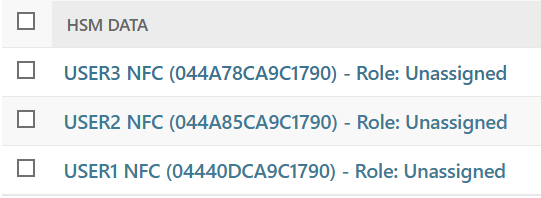
\includegraphics[width=0.9\textwidth]{imaxes/Tests_Users.png}
	\caption{Test Users (1--3) Creation without Role assignation}
	\label{fig:test-users}
\end{figure}

Several CardIDs were first programmed into each card’s NDEF memory using the corresponding modified microcontroller sketch (~\ref{subsubsection:cardidload}). With the MasterKey already loaded into the HSM, the \texttt{/compute\_appkey0/} endpoint was called, sending the message \texttt{READUID1} to derive each card’s AppKey0. Finally, the \texttt{FULL\_ChangeKey} sketch was run on the microcontroller, which authenticates with the MasterKey using the NFC reader and replaces the default card key with the freshly derived AppKey0. After these steps, all cards are fully provisioned and ready for secure operation.

Then, the process defined in the personal authentication data flow (Figure \ref{fig:Personal Auth Data Flow}) starts:
\begin{enumerate}
	\item The USER2 card is approached to the NFC Access Control Unit (NACU) and its NDEF (CardId) file is read (Figure \ref{fig:ndef-read}).
\end{enumerate}

\begin{figure}[H]
	\centering
	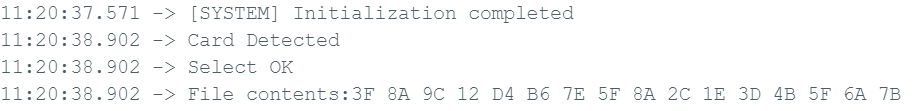
\includegraphics[width=0.9\textwidth]{imaxes/CARDIDREAD}
	\caption{NDEF File Read Integration}
	\label{fig:ndef-read}
\end{figure}

\begin{enumerate}
	\setcounter{enumi}{1}
	\item After the CardId is obtained, it is sent to the ACMS \texttt{/compute\_appkey0/} endpoint through the Wi-Fi module, along with the \texttt{READUID1} message.
	\item AppKey0 is returned to the Wi-Fi module and sent to the microcontroller.
	\item Mutual authentication is performed to read the UID (Figure \ref{fig:mutual-auth}).
\end{enumerate}

\begin{figure}[H]
	\centering
	\includegraphics[width=0.75\textwidth]{imaxes/mutualauth_UID}
	\caption{Mutual Authentication in the Final System}
	\label{fig:mutual-auth}
\end{figure}

\begin{enumerate}
	\setcounter{enumi}{4}
	\item The UID is sent to the \texttt{/submit/} endpoint of the ACMS through the Wi-Fi module.
	\item An authorization message is returned and sent to the microcontroller with a code: 0 for access denied and 1 for access allowed.
	\item The message confirms that the access is denied and the magnetic lock remains locked.
	\item Finally, a mail is sent to the administrator informing of the unauthorized access attempt (Figure \ref{fig:denied-mail}).
\end{enumerate}

\begin{figure}[H]
	\centering
	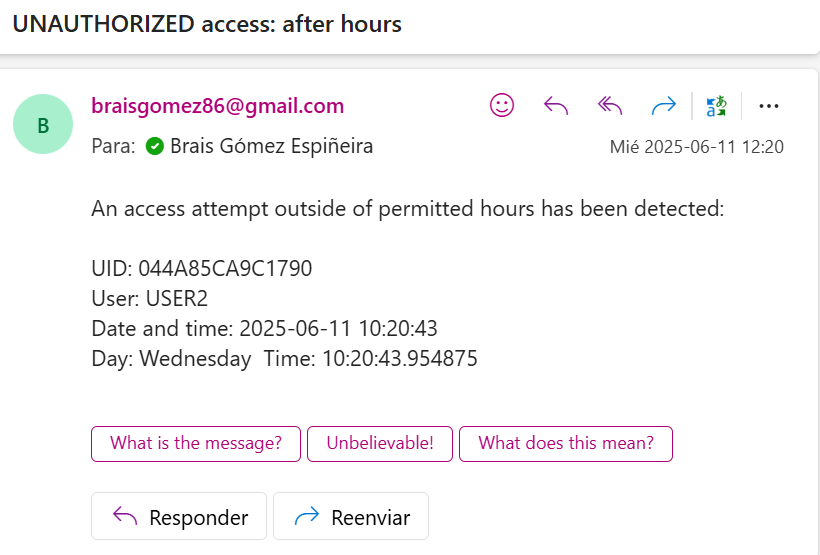
\includegraphics[width=0.75\textwidth]{imaxes/Correo_denegado}
	\caption{Mail Acknowledging Denied Access}
	\label{fig:denied-mail}
\end{figure}
\begin{figure}[H]
	\centering
	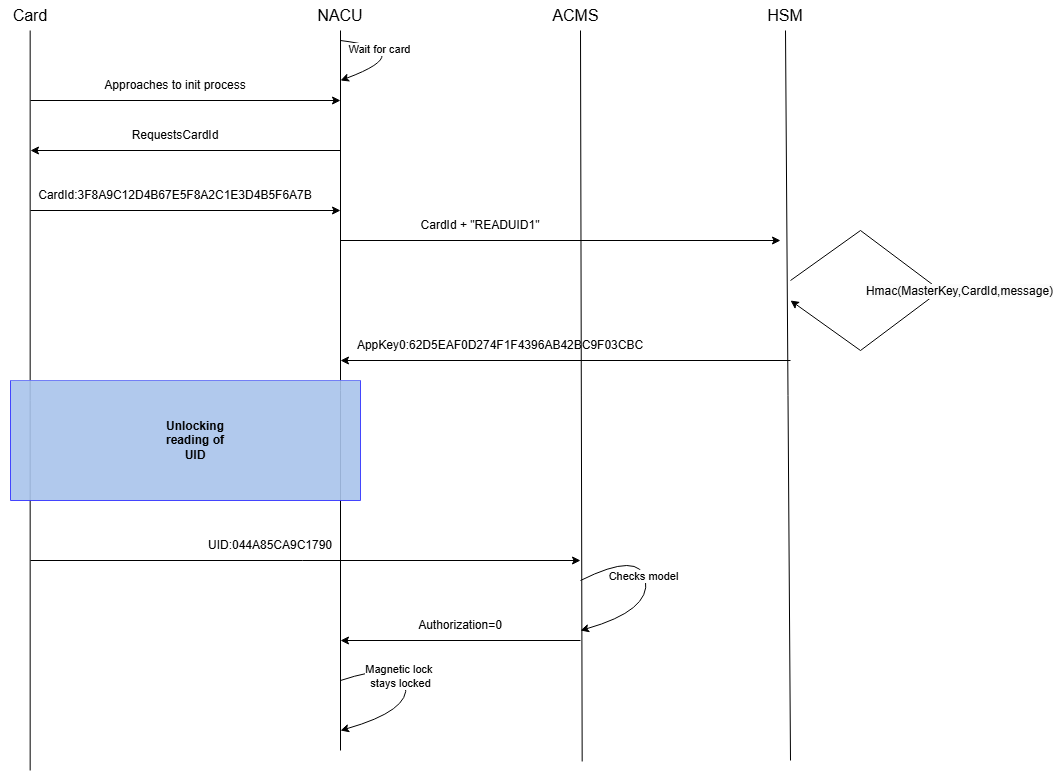
\includegraphics[width=0.75\textwidth]{imaxes/TIDF}
	\caption{Personal authentication data flow for the test case}
	\label{fig:Personal Auth Data Flow}
\end{figure}

USER2 is out of its allowed schedule, which means that the lock does not unlock. Then, the exact same process is repeated with USER1, which is on its allowed schedule, and the lock allows the access as shown in Figure \ref{fig:uid-ok}.

\begin{figure}[H]
	\centering
	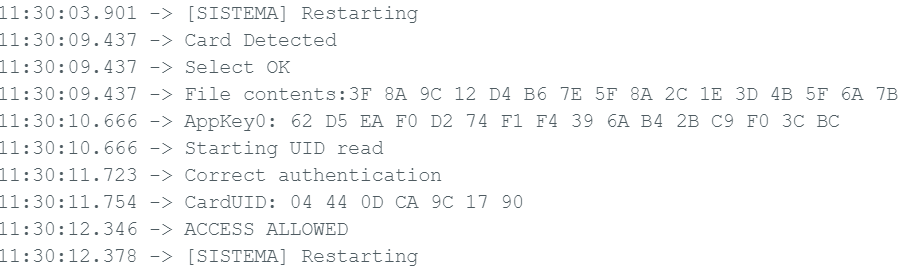
\includegraphics[width=0.9\textwidth]{imaxes/User_Allowed}
	\caption{USER1 Access Allowed Arduino Uno Serial Monitor Data Flow}
	\label{fig:uid-ok}
\end{figure}

\section{Threat Analysis}
\label{sec:threat_analysis}

This project is deeply focused on security, providing confidentiality, authenticity and integrity in identification systems, mitigating threats inherent to the technologies used and IoT environments.

Regarding NFC~\cite{Ref54}, one of the main threats is eavesdropping. Communication between two devices over an NFC channel can be intercepted using several devices such as Flipper Zero or Proxmark 3~\cite{Ref55}, which are designed to exploit vulnerabilities in systems that use ISO 14443A NFC. Although the required physical proximity (less than 10 cm) limits the attack, the use of high-gain antennas or resonant couplings can extend the effective range.

Another risk, related to eavesdropping, is cloning or tag impersonation, which consists in an attacker uploading a stolen NFC tag in another device such as ChameleonMini \cite{Ref57}, trying to impersonate its legit owner. Thanks to mutual authentication, none of these attacks are effective in this system: an attacker could obtain the \texttt{CardId}, but this does not compromise the user nor the whole system. Without access to the HSM it is impossible to derive \texttt{AppKey0}.

There are also interference and denial of service (DoS) attacks that can affect this type of systems. Generating electromagnetic noise in the NFC band or saturating the reader with multiple requests can cause failures or crashes. However, using maglocks ensures that this attack would not let the attacker pass through the protected door. This is because voltage is constantly supplied to the lock, and in order to open it, a voltage cut-off is needed. If the reader were to be saturated, the door would not open because the reader itself would not be able to send the voltage cut-off signal.

In addition, one of the main physical threats is the manipulation of the wiring between Arduino and ESP32, which could lead to data leaks. As this system is designed for academic purposes, wiring is not protected. If this system needs to be installed in a real environment, a proper safe box must be used in order not to be easily manipulated. It is also important to highlight that no key is stored in any of these microcontrollers, as it is considered a malpractice.

Related to the Access Control Management Server (ACMS), several attacks including SQL Injection, XSS in the API, TLS certificate theft, and DoS against the server could be performed. To mitigate these threats, the information that is stored in the Django model database is not critical or personal (e.g., NIF or keys). The NFC tag is stored in it but, again, in case of compromise, it would not be enough to authenticate in the system. Moreover, the \texttt{MasterKey} is stored in a Hardware Security Module to prevent these types of attacks from being effective.

